\documentclass{article}
\usepackage{graphicx}
\usepackage{listings}
\usepackage{color}

\definecolor{dkgreen}{rgb}{0,0.6,0}
\definecolor{gray}{rgb}{0.5,0.5,0.5}
\definecolor{mauve}{rgb}{0.58,0,0.82}
\definecolor{orange}{rgb}{1.0,0.5,0}

\lstset{frame=tb,
  language=Java,
  aboveskip=3mm,
  belowskip=3mm,
  showstringspaces=false,
  columns=flexible,
  basicstyle={\small\ttfamily},
  numbers=none,
  numberstyle=\color{orange},
  keywordstyle=\color{blue},
  commentstyle=\color{dkgreen},
  stringstyle=\color{mauve},
  breaklines=true,
  breakatwhitespace=true,
  tabsize=3
}

\graphicspath{ {out/} }

\title{Analysis of Vector Addition with Threads}
\date{02-03-2016}
\author{Arthur Ceccotti - 8544173}

\begin{document}
  \maketitle

  I have written an implementation of addition of two vectors of random contents using Java (source code on page 3).
  In order to assure correctness of the program, I approached development using the Test Driven Agile methodology with JUnit tests (attached with the code).

  Upon completing the application, I continued by evaluating its performance, running it multiple times with different parameters (number of threads and vector size).
  By attempting to soften intermittent performance drops/spikes, the program was run 20 times, allowing the gathering of average values and standard deviation.

  At first I thought the increase of threads, given constant vector size, would result on a linear increase of performance. Because each thread has equal load (with at most one more operation), vector addition with 4 threads would ideally run twice faster than that with 2 threads of same size. Thus my expected speedup was of \textit{n} times compared to a fully sequential execution, where n is the number of active threads.

  This would certainly not be the case for small vector inputs, given that thread initialisation would be a large overhead.
  Another issue would be executing the program on a single core machine, as threads would never run \textit{truly in parallel} and context switching would be an additinal cost.
  Figure 1 describes the performance decrease given increase of number of threads for a small problem size of 10,000 elements on the machine \textit{mcore48.cs.man.ac.uk}  \footnote{\label{machinespecs} \\
  Dell/AMD quad 12-core (48 cores total), each with specs:\\
  model name: AMD Opteron(tm) Processor 6174 \\
  clock speed: 2.2 GHZ \\
  cache size: 512 KB \\}. I evaluate this to occur mostly due to the thread initialisation cost. As we can see, the program performs much better with a single thread for this problem size, which means in this case it is quicker to do the whole vector addition sequentially, rather than spending a long time spawning threads which will die after doing few operations.
\newpage
\begin{figure}[t]
\centerline{%
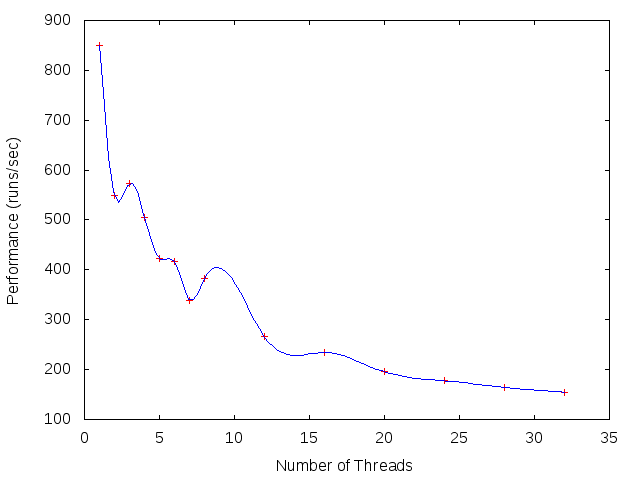
\includegraphics[width=0.56\textwidth]{10k_lines}%
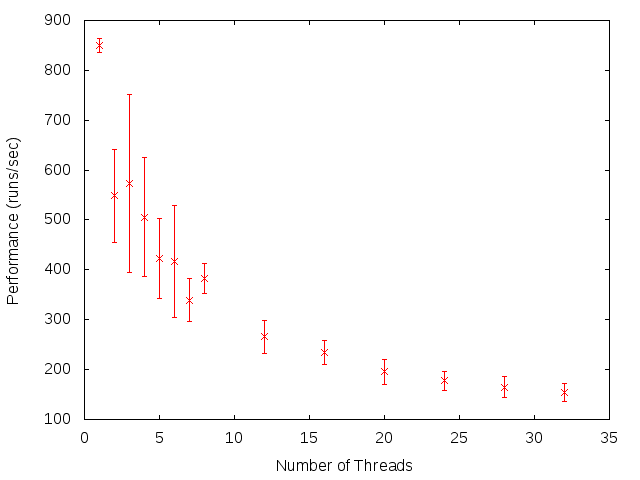
\includegraphics[width=0.56\textwidth]{10k_errorbars}%
}%
\caption{Parallel vector addition of size 10,000. Average performance (left) and standard deviation error range (right) from 20 runs}
\end{figure}
  
  For larger problem sizes (\textgreater1,000,000), thread initialization of a few milliseconds starts becoming insignificant compared to the lifetime of each thread.
  The plot in figure 2 describes the run of my program for the vector size of 10,000,000 with variable threads, where such performance increase is clearly visible.

  This now shows how advantageous multithreaded programming can be for large input problems when few data dependencies are present.

\begin{figure}[t]
\centerline{%
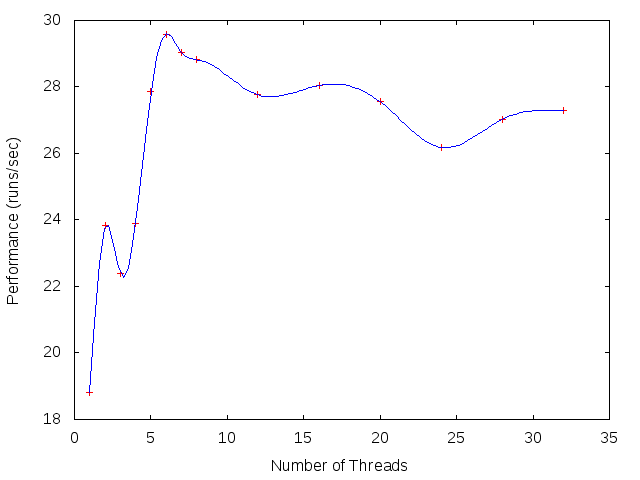
\includegraphics[width=0.56\textwidth]{10M_lines}%
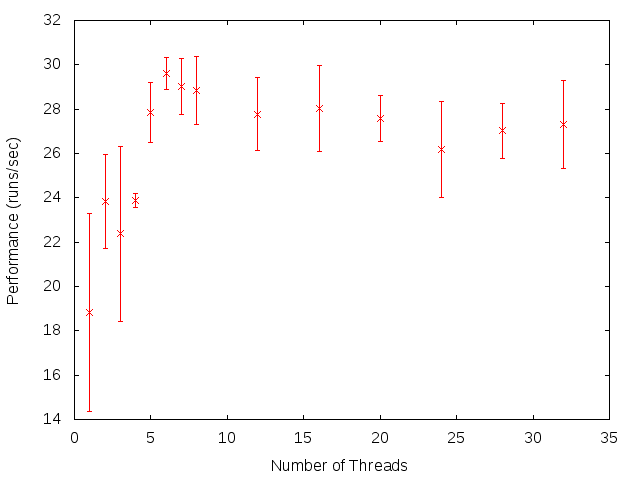
\includegraphics[width=0.56\textwidth]{10M_errorbars}%
}%
\caption{Parallel vector addition of size 10,000,000. Average performance (left) and standard deviation error range (right) from 20 runs}
\end{figure}

\clearpage

\newpage
\newpage\newpage\newpage\newpage
  \lstinputlisting{src/VectorAdder.java}
  \lstinputlisting{src/VectorAdderThread.java}
  \lstinputlisting{src/VectorAdderTest.java}
\end{document}